%% LaTeX Beamer presentation template (requires beamer package)
%% see http://latex-beamer.sourceforge.net/
%% idea contributed by H. Turgut Uyar
%% template based on a template by Till Tantau
%% this template is still evolving - it might differ in future releases!

\documentclass[14pt]{beamer}

\mode<presentation>
{
\usetheme{Berlin}

\setbeamercovered{transparent}
}

\usepackage[ngerman]{babel}
\usepackage[latin1]{inputenc}


% font definitions, try \usepackage{ae} instead of the following
% three lines if you don't like this look
%%%\usepackage{mathptmx}
%%%\usepackage[scaled=.90]{helvet}
%%%\usepackage{courier}

\ifx\pdftexversion\undefined
\usepackage[dvips]{graphicx}
\else
\usepackage{graphicx}
\DeclareGraphicsRule{*}{mps}{*}{}
\fi

%\usepackage[pdftex]{graphicx}
\usepackage{graphics}
%\usepackage{makeidx}
%\usepackage{mathpazo}
%\usepackage{multicol}
%\usepackage{srcltx}
\usepackage{color}
\usepackage{wrapfig}



\title{Magnetische Speichermedien\\ (und deren Ausfallsicherheit)}

%\subtitle{}

% - Use the \inst{?} command only if the authors have different
%   affiliation.
%\author{F.~Author\inst{1} \and S.~Another\inst{2}}
\author{Conrad Kostecki \and Oluf Lorenzen\inst{}}

% - Use the \inst command only if there are several affiliations.
% - Keep it simple, no one is interested in your street address.
\institute
{
\inst \normalfont
Multi Media\\
\normalfont
Berufsbildende Schulen\\
}

\date{LF 4 - Herr Wruck}


% This is only inserted into the PDF information catalog. Can be left
% out.
%%%\subject{Talks}



% If you have a file called "university-logo-filename.xxx", where xxx
% is a graphic format that can be processed by latex or pdflatex,
% resp., then you can add a logo as follows:

\pgfdeclareimage[height=0.5cm]{mmbbslogo}{mmbbslogo}
 \logo{\pgfuseimage{mmbbslogo}}



% Delete this, if you do not want the table of contents to pop up at
% the beginning of each subsection:
%%\AtBeginSubsection[]
%{
%\begin{frame}<beamer>
%\frametitle{Vorgehensweise}
%\tableofcontents[currentsection,currentsubsection]
%\end{frame}
%}

% If you wish to uncover everything in a step-wise fashion, uncomment
% the following command:

%\beamerdefaultoverlayspecification{<+->}

\begin{document}

\begin{frame}
\titlepage
\end{frame}

\begin{frame}
\frametitle{Vorgehensweise}
\tableofcontents
% You might wish to add the option [pausesections]
\end{frame}


\section{Geschichts�berblick}
\begin{frame}
\begin{figure}
 \centering
 \resizebox{!}{120pt}{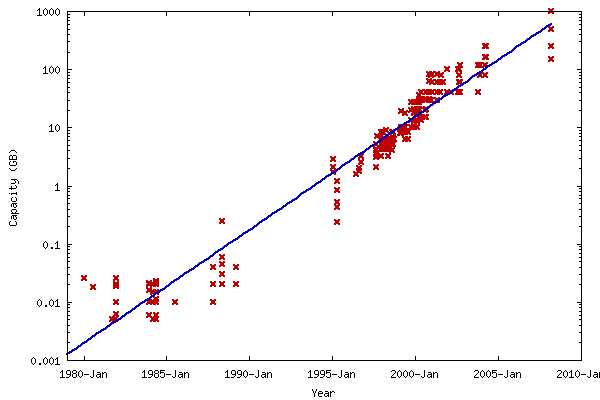
\includegraphics{gfx/Hard_drive_capacity_over_time.png}}
\end{figure}
\begin{itemize}
\item \textbf{1956}: IBM 350 - 5MB - 500kg - 2kW
                % 2 Lesekoepfe fuer kompletten Stapel, 50 Platten
        \item \textbf{2007}: Hitachi - 1TB - 0,7kg - 11W
\end{itemize}
\end{frame}

\begin{frame}
 \frametitle{Formfaktoren}
  \begin{figure}
 \centering
 \resizebox{200pt}{!}{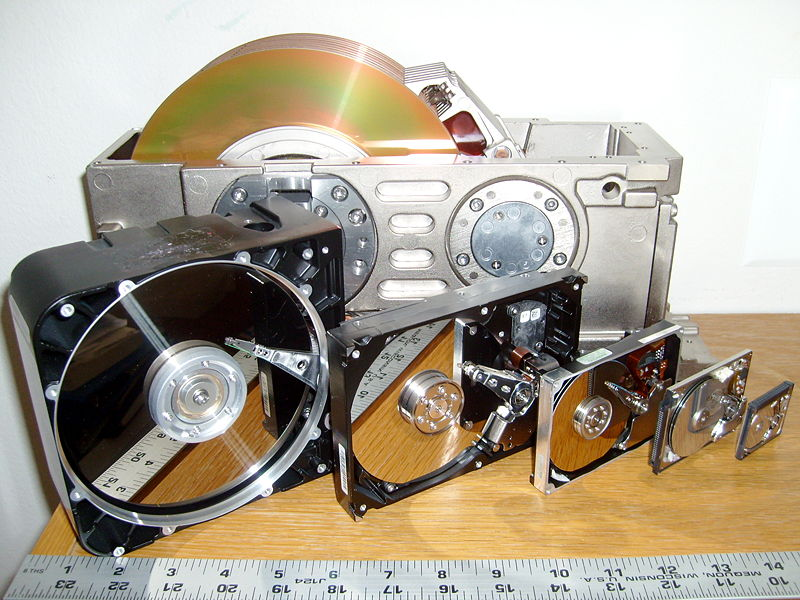
\includegraphics{gfx/800px-SixHardDriveFormFactors.jpg}}
\end{figure}
% 8 inch, 5,25, 3,5, 2,5, 1,8, 1
\end{frame}


\section{Aufbau}
\subsection*{mechanisch}
\begin{frame}

\begin{figure}[h]
 \centering
 \resizebox{240pt}{!}{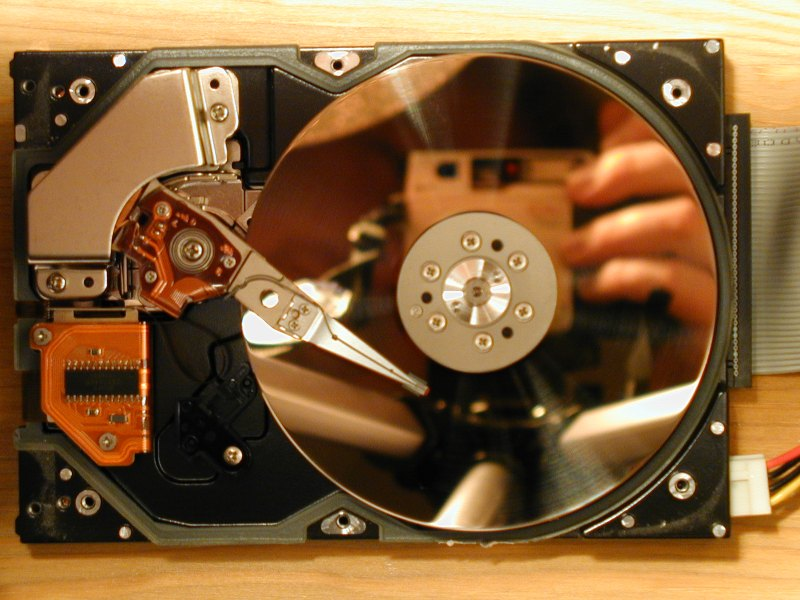
\includegraphics{gfx/harddiskpic.jpg}}
\end{figure}
\end{frame}

\subsection*{logisch}
\begin{frame}

\begin{figure}[h]
 \centering
 \resizebox{80pt}{!}{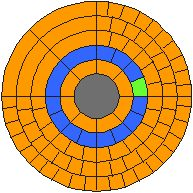
\includegraphics{gfx/hdd_chs.jpg}}
\end{figure}

\begin{itemize}
 \item Scheibe/Platte: 1-4, je nach Kapazit�t
 \item (Lese-) K�pfe: zwei pro Platte
 \item Zylinder/Spur: mehrere Tausend
 \item Sektor: Unterteilung der Zylinder, 512 Byte Nutzdaten
      % plus Pr�fsummen
\end{itemize}
\end{frame}

\subsection*{Kapazit�tssteigerung}
				% 
\begin{frame}
\begin{itemize}
	% GFX
	\item Plotter-Verkleinerung
	\item Perpendicular Recording
\end{itemize}
\end{frame}


\section{Ausfallfaktoren}
				% Blockfehler, defekte Sektoren, Headcrash etc.
				% evtl. Sound-Samples... irgendwer hatte da mal was

\begin{frame}
\begin{itemize}
	\item Temperatur
	\item Headcrash
	\item Mechanik
	\item Elektronik
	\item defekte Sektoren, Blockfehler
\end{itemize}
\end{frame}

\section{Anbindung der Medien}
				% IDE, SCSI, SATA, SAS
\subsection*{alt}
\begin{frame}
\frametitle{P-ATA}
Parallel Integrated Device Electronics
\begin{wrapfigure}{r}{30mm}
 \centering
 \resizebox{80pt}{!}{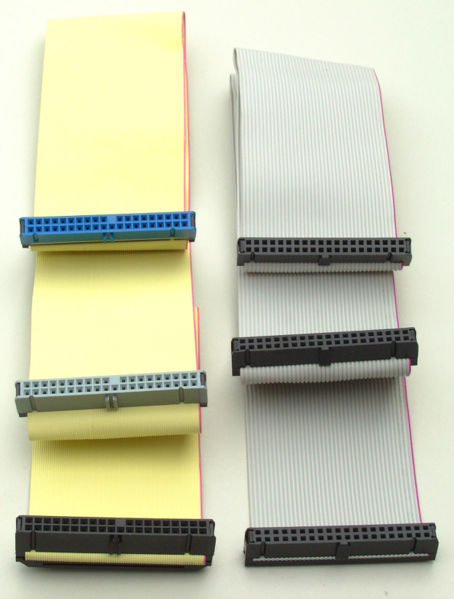
\includegraphics{gfx/454px-IDE_cable_40_pin___80_pin.jpg}}
\end{wrapfigure}

\begin{itemize}
\begin{small}\item ATA-1 (1989)
\item ATA-2 (1994)
\item ATA-3 (1996)
\item ATA-4 / ATAPI-4 (1997)
\item ATA-5 / ATAPI-5 (1999)
\item ATA-6 / ATAPI-6 (2000)
\item ATA-7 / ATAPI-7 (2001)\end{small}
\end{itemize}
\end{frame}

\begin{frame}
 \frametitle{SCSI}
 \textbf{S}mall \textbf{C}omputer \textbf{S}ystem \textbf{I}nterface
 \begin{wrapfigure}{r}{50mm}
 \centering
 \resizebox{120pt}{!}{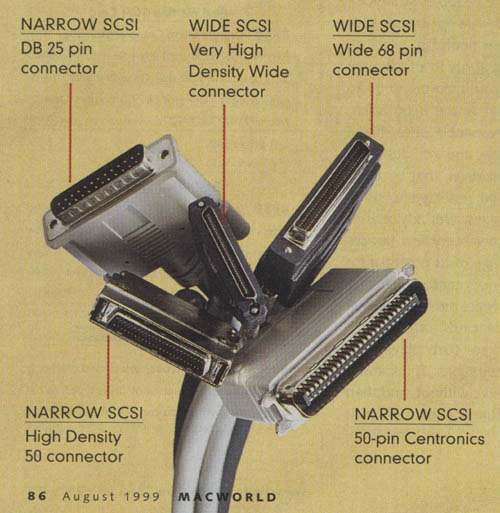
\includegraphics{gfx/scsi.jpg}}
\end{wrapfigure}
\begin{itemize}
\begin{small} \item SCSI-1 (1986)
 \item SCSI-2 (1989)
 \item Ultra-SCSI (1992)
 \item SCSI-3 (1993)
 \item Ultra-2 SCSI (1997)
 \item Ultra-160 (1999)
 \item Ultra-320 (2002)
 \item Sonderform SCA (Single Connector Attachment)\end{small}
\end{itemize}
\end{frame}


\subsection*{neu}
\begin{frame}
 \begin{wrapfigure}{r}{60mm}
 \centering
 \resizebox{160pt}{!}{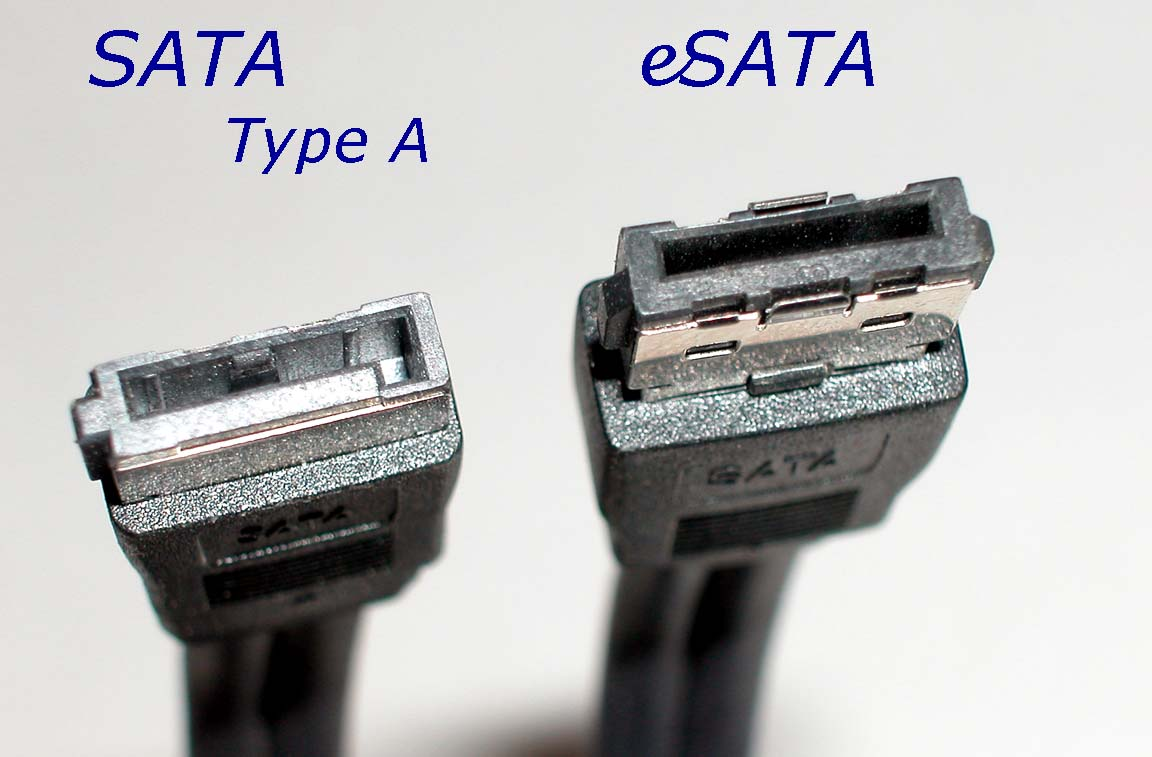
\includegraphics{gfx/eSATA_TypA_lrg.jpg}}
\end{wrapfigure}
\frametitle{S-ATA}
Serial ATA
\begin{itemize}
 \item Serial ATA 1.5 Gbit/s
 \item Serial ATA 3.0 Gbit/s
 \item eSATA
\end{itemize}
\end{frame}

\begin{frame}
  \begin{wrapfigure}{r}{50mm}
 \centering
 \resizebox{160pt}{!}{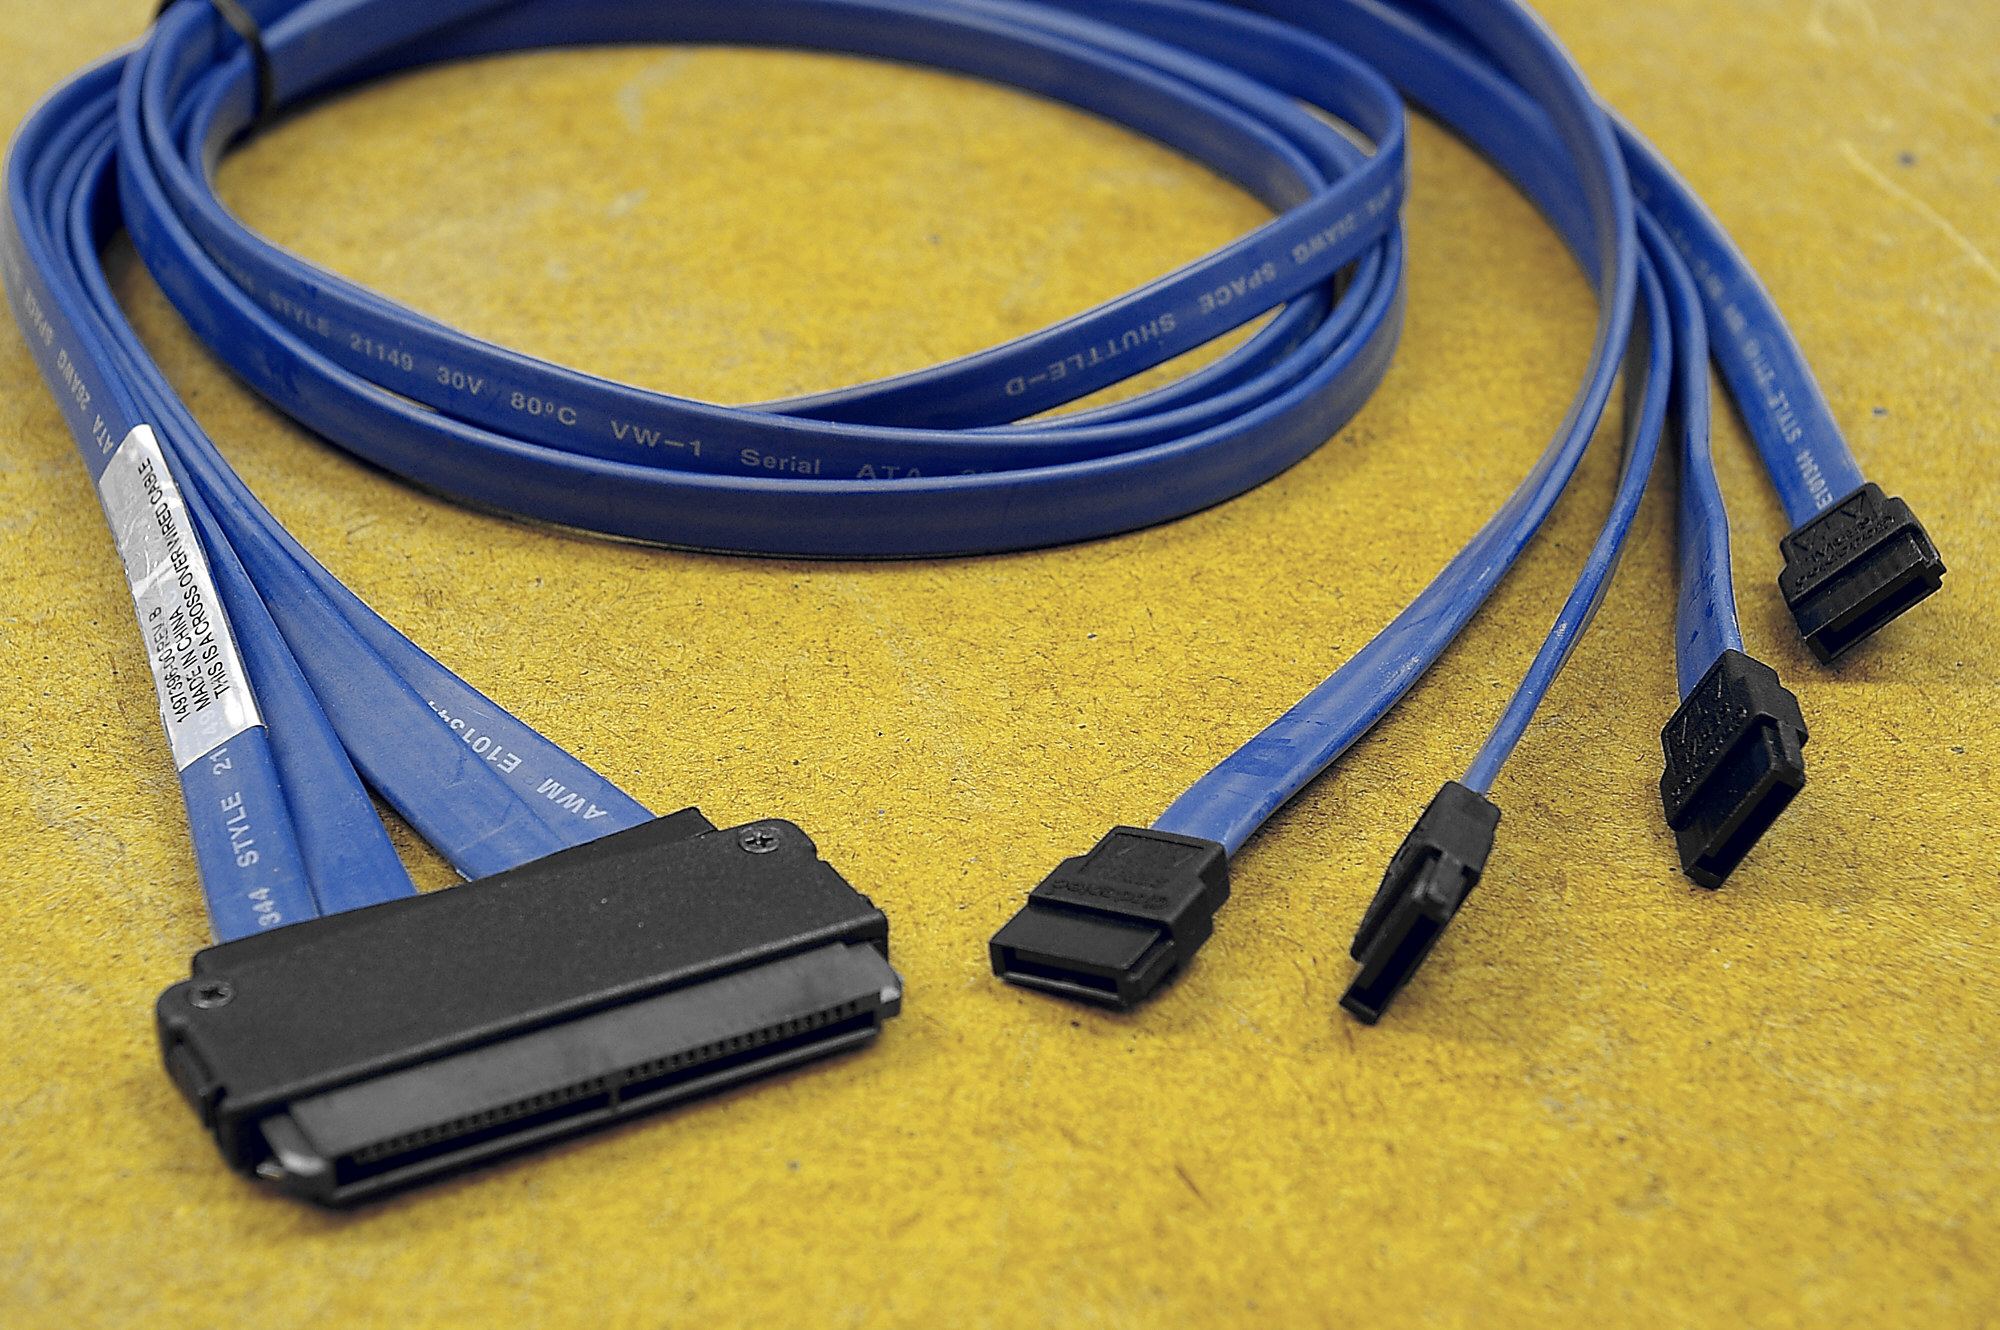
\includegraphics{gfx/SFF-8484_Kabel_IMGP6983.jpg}}
\end{wrapfigure}
 \frametitle{SAS}
 Serial Attatched SCSI
\begin{itemize}
 \item SAS 2.4 Gbit/s
 \item SAS 4.8 Gbit/s
 \item SAS 9.6 Gbit/s
\end{itemize}
\end{frame}


\section{RAID}
\begin{frame}
\textbf{R}edundant \textbf{A}rray of \textbf{I}ndependent \textbf{D}isks;\\
  Urpr�nglich: Redundant Array of Inexpensive Disks
\begin{itemize}
 \item Wurde erstmals 1987 von Gibson und Katz Patterson verwendet
 \item Erh�hung der Ausfallsicherheit
 \item Steigerung der Geschwindigkeit
 \item Austausch von Festplatten w�hrend des Betriebs
 \item Preisvorteil durch mehrere kleine Festplatten
\end{itemize}
\end{frame}
				% softraid-hardraid, RaidX, Raid XY

%\subsection{Pseudo- und Hardware-RAID}
%\subsection{single- und double-RAID}
%\begin{frame}
%\frametitle{ \textbf{R}edundant \textbf{A}rray of \textbf{I}ndependent \textbf{D}isks}
%\begin{itemize}
%	\item genereller Aufbau
%\end{itemize}
%\end{frame}

\subsection*{RAID 0}
\begin{frame}
\begin{figure}
 \centering
 \resizebox{100pt}{!}{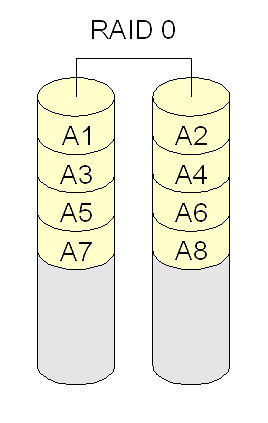
\includegraphics{gfx/RAID_0.png}}
\end{figure}

\end{frame}

\subsection*{RAID 1}
\begin{frame}
\begin{figure}
 \centering
 \resizebox{100pt}{!}{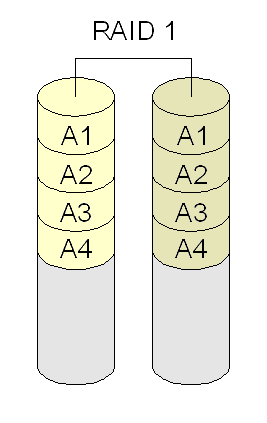
\includegraphics{gfx/RAID_1.png}}
\end{figure}
\end{frame}

\subsection*{RAID 5}
\begin{frame}
\begin{figure}
 \centering
 \resizebox{200pt}{!}{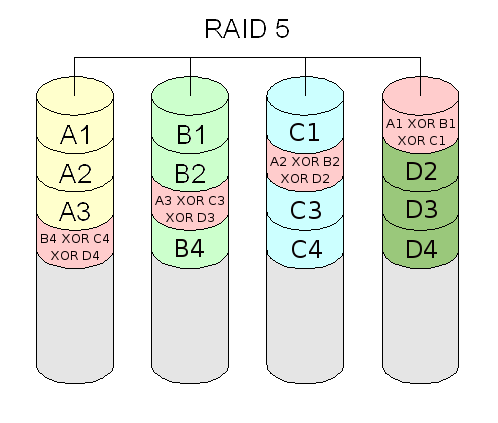
\includegraphics{gfx/RAID_5.png}}
\end{figure}
\end{frame}

\subsection*{RAID 0+1}
\begin{frame}
\begin{figure}
 \centering
 \resizebox{180pt}{!}{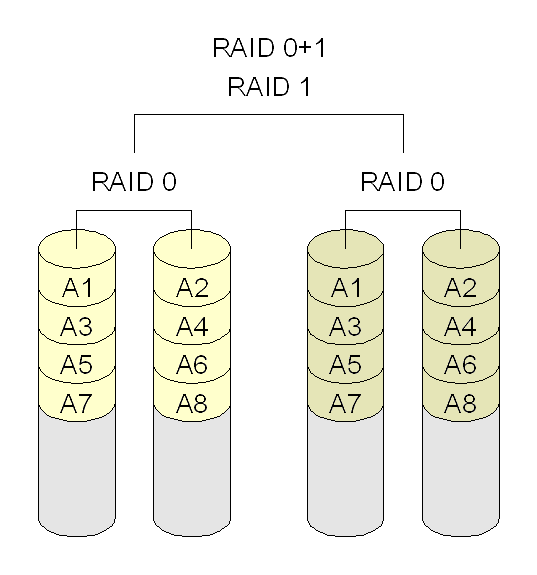
\includegraphics{gfx/RAID_01.png}}
\end{figure}
\end{frame}


\section{Bandlaufwerke}
\begin{frame}
  \begin{wrapfigure}{r}{50mm}
 \centering
 \resizebox{160pt}{!}{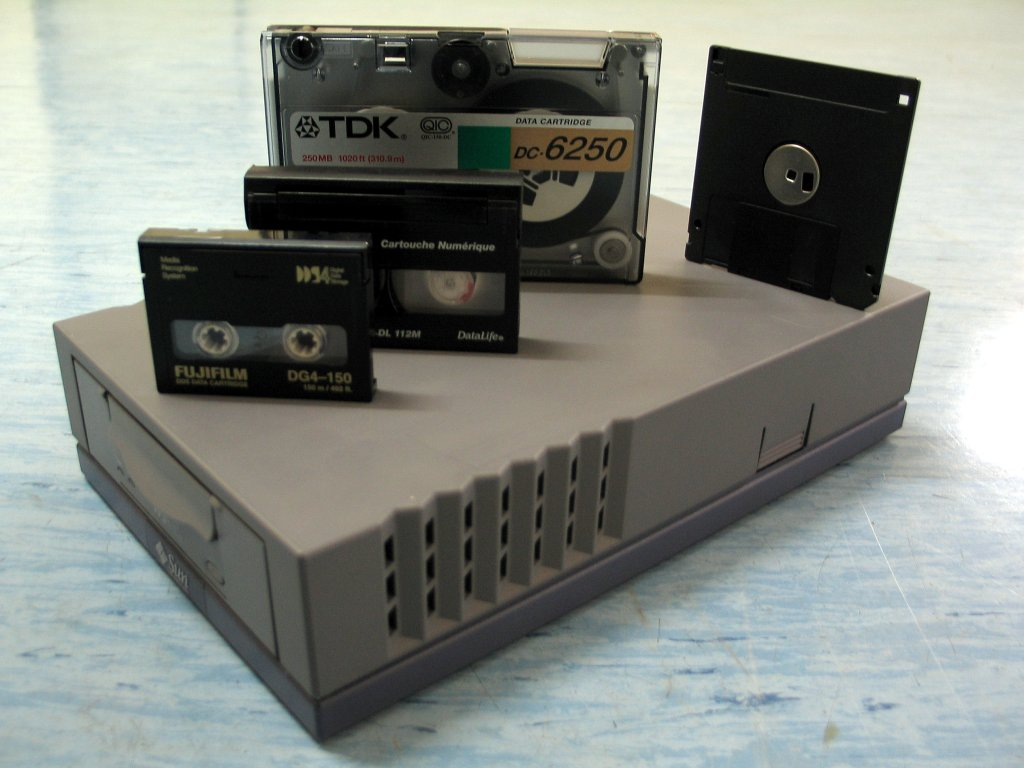
\includegraphics{gfx/Dds_tape_drive_01.jpg}}
\end{wrapfigure}
Vorteile:
\begin{footnotesize}\begin{itemize}
	\item Kapazit�t
	\item Lebensdauer
        \item Platz
        \item Kosten
        \item Geschwindigkeit
\end{itemize}             \end{footnotesize}

Nachteile:
\begin{footnotesize}  \begin{itemize}
   \item Empfindlichkeit
   \item Geschwindigkeit
  \end{itemize}\end{footnotesize}

\end{frame}

\section[]{}
\begin{frame}
  % wikipedia ist ein anfang-hinweis
\begin{itemize}
 \item wikipedia.org
 \begin{itemize}
  \item Harddisk
  \item Perpendicular recording
  \item Superparamagnetism
 \end{itemize}
\item pcworld.com
\item hardwarezone.com
\item hitachigst.com
\item ibm.com
\item quantum.com
\end{itemize}
  \vskip0pt plus.5fill
  \begin{scriptsize}\ldots erstellt mit \LaTeX\end{scriptsize}
\end{frame}


\section[]{}
\begin{frame}
\begin{center}\Large Vielen Dank f\"{u}r\\eure Aufmerksamkeit \& Kritik!\end{center}
\end{frame}


\end{document}
